%
%  Erik Olsen
%
\documentclass[12pt,fullpage]{article}
\usepackage{fullpage}                                        % use all of the page for text 
\usepackage{psfrag}                                          % LaTeX graphics tool
\usepackage{pslatex}                                         % avoids the default cmr font
\usepackage{graphicx}                                        % graphics package 
\usepackage{epsfig}                                          % figures
\usepackage{epsfig} 
\usepackage{hyperref}
\usepackage{color}

\begin{document}

\noindent
{\bf Standard uniform distribution} (from \color{blue}\url{http://www.math.wm.edu/~leemis/chart/UDR/UDR.html}\color{black})

\noindent
The shorthand $X \sim U(0,1)$ is used to indicate that the
random variable $X$ has the standard uniform distribution with minimum 0 and maximum 1.
A standard uniform random variable $X$ has probability density function 
$$
f(x) = 1\qquad \qquad 0 < x < 1.
$$
The standard uniform distribution is central to random variate generation.
The probability density function is illustrated below.
{\begin{figure}[h!]
\begin{center}
\psfrag{labx}{$x$}
\psfrag{labf}{$f(x)$}
\psfrag{laba}{$0$}
\psfrag{labb}{$1$}
\psfrag{labff}{$1$}
\includegraphics[width=3.2in]{StandarduniformPlot.ps}
\end{center}
\end{figure}}

\noindent
The cumulative distribution function on
the support of $X$ is
$$
F(x) = P(X \le x) = x \qquad \qquad 0 < x < 1.
$$
The survivor function on the support of $X$ is
$$
S(x) = P(X \ge x) = 1- x \qquad \qquad 0 < x < 1.
$$
The hazard function on the support of $X$ is
$$
h(x) = \frac{f(x)} {S(x)} =\frac{1}{1 - x} \qquad \qquad 0 < x < 1.
$$
The cumulative hazard function on the support of $X$ is
$$
H(x) = - \ln \,S(x) =  - \ln(1 - x) \qquad \qquad 0 < x < 1.
$$
The inverse distribution function of $X$ is
$$
F ^ {-1}(u) = u \qquad \qquad 0 < u < 1.
$$
The median of $X$ is $1/2$.

\noindent
The moment generating function of $X$ is
$$
M(t) = \left\{ \begin{array}{ll} 
       1 & \qquad t = 0\\ 
      \frac{e^{\kern 0.04em t}-1}{t} & \qquad t \neq 0
       \end{array} \right.
$$
The characteristic function of $X$ is
$$
\phi(t) = \left\{ \begin{array}{ll} 
          1 & \qquad t = 0\\ 
         \frac{e^{\kern 0.04em it}-1}{it} & \qquad t \neq 0
          \end{array} \right.
$$
The population mean, variance, skewness and kurtosis of $X$ are
$$
E[X] = \frac{1}{2} \qquad \qquad 
V[X] = \frac{1}{12} \qquad \qquad
E\left[ \left( \frac{X - \mu}{\sigma} \right) ^ {\kern -0.08 em 3} \right] = 0 \qquad \qquad 
E\left[ \left( \frac{X - \mu}{\sigma} \right) ^ {\kern -0.08 em 4} \right] = \frac{9}{5}.
$$


\vspace{0.1in}

\noindent
{\bf APPL verification:}
The APPL statements
\begin{verbatim}
X := UniformRV(0,1);
Mean(X);
Variance(X);
Skewness(X);
Kurtosis(X);
MGF(X);
\end{verbatim}
verify the population mean, variance, skewness, kurtosis, and moment generating function.
\end{document}
